\section{Post-Fabrication-Tunable Time-Domain Read}
\label{sec:read}
\begin{figure}[!t]
\centering
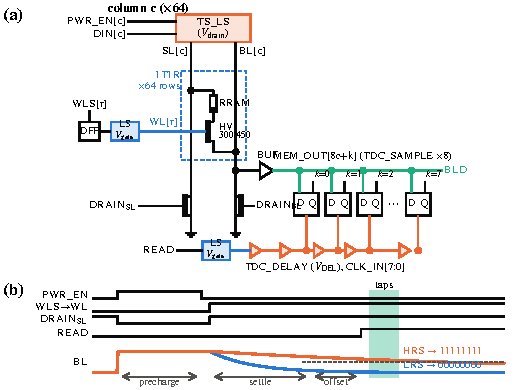
\includegraphics[width=\columnwidth]{schematic}
\caption{(a) One column of the macro with its TDC. (b) Read sequence, with the eight-tap window shaded.}
\label{fig:schematic}
\end{figure}
If the model cannot say where the fabricated cells will sit, the read circuit has to be able to find them, and this section proposes a read built around that requirement.
Fig.~\ref{fig:schematic} shows the proposed post-fabrication-tunable time-domain readout circuit and its read sequence.
A conventional sense amplifier asks whether the bit line is above or below a reference at one instant, whereas this read asks how long the bit line takes to discharge.
A read precharges the bit line BL to the drive voltage $\Vd$, opens the selected rows, and then grounds the source line SL, so that BL discharges through the selected cells with a time constant set by the cell resistance, the access-transistor resistance, and the bit-line capacitance.
A buffer with a threshold of about 0.6\,V converts BL into a digital signal, and eight flip-flops sample this signal on the eight taps of a delay line that a READ pulse triggers.
The result is a thermometer code that counts the taps at which BL was still high, so that a low-resistance (LRS) cell gives a short code and a high-resistance (HRS) cell a long one (Fig.~\ref{fig:schematic}(b)).

Three knobs place the decision, and none of them is a transistor size.
The controller inserts a signed offset between the grounding of SL and the READ pulse in 10\,ns steps, which moves the sampling window along the discharge; a dedicated supply pad $\Vdel$ sets the delay of the line and with it the tap pitch; and the word-line supply $\Vg$ sets the access-transistor resistance together with the level-shifter delay.
All three are registers or pads, so the window can be placed after the resistance and the capacitance of the fabricated cells have been measured, and no reference cell has to be programmed with the same uncertain device.

With $n$ rows open, the column conductance is the sum of the selected cells, so the discharge time, and with it the code $c(k)$, falls monotonically with the number $k$ of LRS cells among them.
The in-memory operations are thresholds on this code, each with a margin measured in taps.
A NOR over the $n$ rows separates $k=0$ from $k\ge1$ with a margin of $c(0)-c(1)$, and a majority separates $k\le n/2$ from $k>n/2$ with a margin of $c(n/2)-c(n/2+1)$.
These bitwise operations over an arbitrary row mask are the primitive of digital PiM~\cite{li2016pinatubo}, and here they come out of the same read that serves a single row.
